\documentclass[12pt,fleqn]{article}\usepackage{../common}
\begin{document}
Naive Bayes

Reel sayilar arasinda baglanti kurmak icin istatistikte regresyon
kullanilir. Eger reel degerleri, (mesela) iki kategorik grup arasinda secmek
icin kullanmak istenirse, bunun icin lojistik regresyon gibi teknikler de
vardir.

Fakat kategoriler / gruplar ile baska kategorik gruplar arasinda
baglantilar kurulmak istenirse, standart istatistik yontemleri faydali
olamiyor. Bu gibi ihtiyaclar icin makine ogrenimi (machine learning)
dunyasindan Naive Bayes gibi tekniklere bakmamiz lazim.

Not: Daha ilerlemeden belirtelim, bu teknigin ismi Naive Bayes ama bu tanim
dogru degil, cunku bu teknik Olasilik Teorisi'nden bilinen Bayes Teorisini
kullanmiyor.

Oncelikle kategorik degerler ile ne demek istedigimizi belirtelim. Reel
sayilar $0.3423, 2.4334$ gibi degerlerdir, kategorik degerler ile ise
mesela bir belge icinde 'a','x' gibi harflerin mevcut olmasidir. Ya da, bir
evin 'beyaz', 'gri' renkli olmasi.. Burada oyle kategorilerden bahsediyoruz
ki istesek te onlari sayisal bir degere ceviremiyoruz; kiyasla mesela bir
gunun 'az sicak', 'orta', 'cok sicak' oldugu verisini kategorik bile olsa
regresyon amaciyla sayiya cevirip kullanabilirdik. Az sicak = 0, orta = 1,
cok sicak = 2 degerlerini kullanabilirdik, regresyon hala anlamli olurdu
(cunku arka planda bu kategoriler aslinda sayisal sicaklik degerlerine
tekabul ediyor olurlardi). Fakat 'beyaz', 'gri' degerlere sayi atamanin
regresyon acisindan bir anlami olmazdi, hatta bunu yapmak yanlis
olurdu. Eger elimizde fazla sayida 'gri' ev verisi olsa, bu durum regresyon
sirasinda beyaz evlerin beyazligini mi azaltacaktir?

Iste bu gibi durumlarda kategorileri oldugu gibi isleyebilen bir teknik
gerekiyor. Bu yazida kullanacagimiz ornek, bir belgenin icindeki kelimelere
gore kategorize edilmesi. Elimizde iki turlu dokuman olacak. Bir tanesi
Stephen Hawking adli bilim adaminin bir kitabindan 3 sayfa, digeri baskan
Barack Obama'nin bir kitabindan 3 sayfa. Bu sayfalar ve icindeki kelimeler
NB yontemini "egitmek" icin kullanilacak, sonra NB tarafindan hic
gorulmemis yeni sayfalari yontemimize kategorize ettirecegiz.

Cok Boyutlu Bernoulli ve Kelimeler

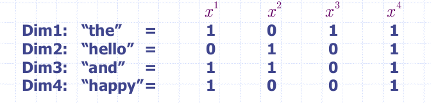
\includegraphics[height=4cm]{dims.png}

Bir dokuman ile icindeki kelimeler arasinda nasil baglanti kuracagiz?
Burada olasilik teorisinden Cok Boyutlu Bernoulli (Multivariate Bernoulli)
dagilimini kullanacagiz. Ustteki resimde goruldugu gibi her dokuman bir
$x^i$ rasgele degiskeniyle temsil edilecek. Tek boyutlu Bernoulli degiskeni
'1' ya da '0' degerine sahip olabilir, cok boyutlu olani ise bir vektor
icinde '1' ve '0' degerlerini tasiyabilir. Iste bu vektorun her hucresi,
onceden tanimli bir kelimeye tekabul edecek, ve bu kelimeden bir dokuman
icinde en az bir tane var ise, o hucre '1' degerini tasiyacak, yoksa '0'
degerini tasiyacak. Ustteki ornekte 2. kelime "hello" ve 4. dokuman
icinde bu kelimeden en az bir tane var, o zaman $x_2^4 = 1$. Tek bir
dokumani temsil eden dagilimi matematiksel olarak soyle yazabiliriz:

$$ p(x_1,...,x_{D}) = \prod_{d=1}^{D} p(x_d)=\prod_{d=1}^{D}
\alpha_d^{x_d}(1-\alpha_d)^{1-x_d} 
$$

Bu formulde her $d$ boyutu bir tek boyutlu Bernoulli, ve bir dokuman
icin tum bu boyutlarin ortak (joint) dagilimi gerekiyor, carpimin
sebebi bu. Formuldeki $\alpha_d$ bir dagilimi "tanimlayan" deger,
$\alpha$ bir vektor, ve unutmayalim, her "sinif" icin NB ayri ayri
egitilecek, ve her sinif icin farkli $\alpha$ vektoru olacak. Yani
Obama'nin kitaplari icin $\alpha_2 = 0.8$ olabilir, Hawking kitabi
icin $\alpha_2 = 0.3$ olabilir. Birinin kitabinda "hello" kelimesi
olma sansi fazla, digerinde pek yok. O zaman NB'yi "egitmek" ne
demektir? Egitmek her sinif icin yukaridaki $\alpha$ degerlerini
bulmak demektir.

Bunun icin istatistikteki "olurluk (likelihood)" kavramini kullanmak
yeterli. Olurluk, bir dagilimdan geldigi farzedilen bir veri setini
alir, tum veri noktalarini teker teker olasiliga gecerek olasilik
degerlerini birbirine carpar. Sonuc ne kadar yuksek cikarsa, bu
verinin o dagilimdan gelme olasiligi o kadar yuksek demektir. Bizim
problemimiz icin tek bir sinifin olurlugu, o sinif icindeki tum (N
tane) belgeyi kapsamalidir, tek bir "veri noktasi" tek bir belgedir,
o zaman:

$$ L(\theta) = \prod_{i=1}^N \prod_{d=1}^{D} p(x_d^i) = 
\prod_{i=1}^N \prod_{d=1}^{D} \alpha_d^{x_d^i}(1-\alpha_d)^{1-x_d^i}
 $$

$\theta$ bir dagilimi tanimlayan her turlu degisken anlaminda kullanildi, bu
ornekte icinde sadece $\alpha$ var.

Devam edelim: Eger $\alpha$'nin ne oldugunu bilmiyorsak (ki bilmiyoruz
-egitmek zaten bu demek-) o zaman maksimum olurluk (maximum likelihood)
kavramini resme dahil etmek gerekli. Bunun icin ustteki olurluk formulunun
$\alpha$'ya gore turevini alip sifira esitlersek, bu formulden bir maksimum
noktasindaki $\alpha$ elimize gececektir. Iste bu $\alpha$ bizim aradigimiz
deger. Veriyi en iyi temsil eden $\alpha$ degeri bu demektir. Onu bulunca
egitim tamamlanir.

Turev almadan once iki tarafin log'unu alalim, boylece carpimlar toplamlara
donusecek ve turevin formulun icine nufuz etmesi daha kolay olacak.

$$ \log(L) = \sum_{i=1}^N \sum_{d=1}^{D} {x_d^i}\ log (\alpha_d) + 
(1-x_d^i)\ log (1-\alpha_d) $$

Turevi alalim:

$$ \frac{dlog(L)}{d\alpha_d} = \sum_{i=1}^N \bigg( \frac{x_d^i}{\alpha_d} -
\frac{1-x_d^i}{1-\alpha_d} \bigg) = 0
 $$

1- $\alpha_d$'ye gore turev alirken $x_d^i$'ler sabit sayi gibi muamele
gorurler. 2- log'un turevi alirken log icindeki degerlerin turev alinmis hali
bolumun ustune, kendisini oldugu gibi bolum altina alinir, ornek 
$dlog(-x)/dx = -1/x$ olur ustteki eksi isaretinin sebebi bu. 

Peki $\sum_{d=1}^{D}$ nereye gitti? Turevi $\alpha_d$'ye gore aliyoruz ve o
turevi alirken tek bir $\alpha_d$ ile ilgileniyoruz, mesela $\alpha_{22}$,
bunun haricindeki diger tum $\alpha_?$ degerleri turev alma islemi
sirasinda sabit kabul edilirler, turev sirasinda sifirlanirlar. Bu sebeple
$\sum_{d=1}^{D}$ icinde sadece bizim ilgilendigimiz $\alpha_d$ geriye
kalir. Tabii ki bu ayni zamanda her $d=1,2,..D$, $\alpha_d$ icin ayri bir
turev var demektir, ama bu turevlerin hepsi birbirine benzerler, yani tek
bir $\alpha_d$'yi cozmek, hepsini cozmek anlamina gelir.

Devam edelim:

$$ \sum_{i=1}^N \bigg( \frac{x_d^i}{\alpha_d} - \frac{1-x_d^i}{1-\alpha_d} \bigg) =
\frac{N_d}{\alpha_d} - \frac{N-N_d}{1-\alpha_d} = 0
 $$

$\sum_{i=1}^N x_d^i = N_d$ olarak kabul ediyoruz, $N_d$ tum veri icinde $d$
boyutu (kelimesi) '1' kac tane hucre oldugunu bize soyler. $x_d^i$ ya '1' ya '0'
olabildigine gore bir $d$ icin, tum $N$ hucrenin toplami otomatik olarak bize
kac tane '1' oldugunu soyler. Sonra:

$$ \frac{N_d}{\alpha_d} - \frac{N-N_d}{1-\alpha_d} = 0  $$

$$ \frac{1-\alpha_d}{\alpha_d} = \frac{N-N_d}{N_d}   $$

$$ \frac{1}{\alpha_d} - 1 = \frac{N}{N_d} - 1  $$

$$ \frac{1}{\alpha_d} = \frac{N}{N_d}  $$

$$ \alpha_d = \frac{N_d}{N}  $$

Python Kodu

$\alpha_d$'nin formulunu buldumuza gore artik kodu yazabiliriz. Ilk once bir
dokumani temsil eden cok boyutlu Bernoulli vektorunu ortaya cikartmamiz
lazim. Bu vektorun her hucresi belli bir kelime olacak, ve o kelimelerin ne
oldugunu onceden kararlastirmamiz lazim. Bunun icin her siniftaki tum
dokumanlardaki tum kelimeleri iceren bir sozluk yaratiriz:

\begin{minted}{python}
import re
import math

words = {}

# find all words in all files, creating a 
# global dictionary.
for file in ['a1.txt','a2.txt','a3.txt',
             'b1.txt','b2.txt','b3.txt']:
    f = open (file)
    s = f.read()
    tokens = re.split('\W+', s)
    for x in tokens: words[x] = 0.
    
hawking_alphas = words.copy()   
for file in ['a1.txt','a2.txt','a3.txt']:
    words_hawking = set()
    f = open (file)
    s = f.read()
    tokens = re.split('\W+', s)
    for x in tokens: 
        words_hawking.add(x)
    for x in words_hawking:
        hawking_alphas[x] += 1.
        
obama_alphas = words.copy()   
for file in ['b1.txt','b2.txt','b3.txt']:
    words_obama = set()
    f = open (file)
    s = f.read()
    tokens = re.split('\W+', s)
    for x in tokens: 
        words_obama.add(x)
    for x in words_obama:
        obama_alphas[x] += 1.

for x in hawking_alphas.keys():
    hawking_alphas[x] = hawking_alphas[x] / 3.        
for x in obama_alphas.keys():
    obama_alphas[x] = obama_alphas[x] / 3.        

def prob(xd, alpha):
    return math.log(alpha*xd + 1e-10) + \
        math.log((1.-alpha)*(1.-xd) + 1e-10)
        
def test(file):
    test_vector = words.copy()   
    words_test = set()
    f = open (file)
    s = f.read()
    tokens = re.split('\W+', s)
    for x in tokens: 
        words_test.add(x)
    for x in words_test:  
        test_vector[x] = 1.
    ob = 0.
    ha = 0.
    for x in test_vector.keys(): 
        if x in obama_alphas: 
            ob += prob(test_vector[x], obama_alphas[x])
        if x in hawking_alphas: 
            ha += prob(test_vector[x], hawking_alphas[x])
                
    print "obama", ob, "hawking", ha, \
    "obama", ob > ha, "hawking", ha > ob


print "hawking test"    
test('a4.txt')
print "hawking test"    
test('a5.txt')
print "obama test"    
test('b4.txt')
print "obama test"    
test('b5.txt')
\end{minted}

\begin{verbatim}
hawking test
obama -34048.7734496 hawking -32192.3692113 obama False hawking True
hawking test
obama -33027.3182425 hawking -32295.7149639 obama False hawking True
obama test
obama -32531.9918709 hawking -32925.037558 obama True hawking False
obama test
obama -32205.4710748 hawking -32549.6924713 obama True hawking False
\end{verbatim}

Test icin yeni dokumani kelimelerine ayiriyoruz, ve her kelimeye tekabul eden
alpha vektorlerini kullanarak bir yazar icin toplam olasiligi
hesapliyoruz. Nasil? Her kelimeyi $\alpha_d^{x_d}(1-\alpha_d)^{1-x_d}$ formulune
soruyoruz, yeni dokumani temsilen elimizde bir $[1,0,0,1,0,0,...,1]$ seklinde
bir vektor oldugunu farz ediyoruz, buna gore mesela $x_1=1$, $x_2=0$. Eger bir
$d$ kelimesi yeni belgede "var" ise o kelime icin $x_d = 1$ ve bu durumda
$\alpha_d^{x_d} = \alpha_d^{1} = \alpha_d$ haline gelir, ama formulun oteki
tarafi yokolur, $(1-\alpha_d)^{1-x_d} = (1-\alpha_d)^0 = 1$, o zaman $\alpha_d
\cdot 1 = \alpha_d$.

Carpim diyoruz ama biz aslinda siniflama sirasinda
$\alpha_d^{x_d}(1-\alpha_d)^{1-x_d}$ carpimi yerine yine log() numarasini
kullandik; cunku olasilik degerleri hep 1'e esit ya da ondan kucuk sayilardir,
ve bu kucuk degerlerin birbiriyle surekli carpimi nihai sonucu asiri fazla
kucultur. Asiri ufak degerlerle ugrasmamak icin olasiliklarin log'unu alip
birbirleri ile toplamayi sectik, yani hesapladigimiz deger $x_d \cdot
log(\alpha_d) + (1-x_d) \cdot \log(1-\alpha_d)$

Fonksiyon \verb!prob! icindeki \verb!1e-7! kullanimi neden? Bu
kullanim log numarisini yapabilmek icin -- sifir degerinin log degeri
tanimsizdir, bir kelime olmadigi zaman log'a sifir gelecegi icin hata
olmamasi icin log icindeki degerlere her seferinde yeterince kucuk bir
sayi ekliyoruz, boylece pur sifirla ugrasmak zorunda kalmiyoruz. Sifir
olmadigi zamanlarda cok eklenen cok kucuk bir sayi sonucta buyuk
farklar (hatalar) yaratmiyor.

Toparlarsak, yeni belge \verb!a4.txt! icin iki tur alpha
degerleri kullanarak iki farkli log toplamini hesaplatiyoruz. Bu iki
toplami birbiri ile karsilastiriyoruz, hangi toplam daha buyukse,
dokumanin o yazardan gelmesi daha olasidir, ve o secimimiz o yazar
olur.

Anahtarlama (Hashing) Numarasi

Ustteki kodda bir problem var, dokumani temsil eden ve icinde 1 ya da
0 hucreli ozellik vektorunu (feature vector) olusturmak icin tum
kelimelerin ne oldugunu bilmeliyiz. Yani veriyi bir kere bastan sonra
tarayarak bir sozluk olusturmaliyiz (ki oyle yapmaya mecbur kaldik) ve
ancak ondan sonra her dokuman icin hangi kelimenin olup olmadigini
saptamaya ve onu kodlamaya baslayabiliriz. Halbuki belgelere bakar
bakmaz, teker teker giderken bile hemen bir ozellik vektoru
olusturabilseydik daha iyi olmaz miydi?

Bunu basarmak icin anahtarlama numarasini kullanmamiz lazim. Bilindigi
gibi temel yazilim bilime gore bir kelimeyi temsil eden bir anahtar
(hash) uretebiliriz, ki bu hash degeri bir sayidir. Elimizde bir
"sayi" olmasi bize faydali olur yarar, bu sayinin en fazla kac
olabileceginden hareketle (hatta bu sayiya bir limit koyarak) ozellik
vektorumuzun boyutunu onceden saptamis oluruz.  Sonra kelimeye
bakariz, hash uretiriz, sonuc mesela 230 geldi, o zaman ozellik
vektorundeki 230'uncu kolonun degerini 1 yapariz. 

\begin{minted}{python}
d_input = dict()

def add_word(word):
    hashed_token = hash(word) % 127
    d_input[hashed_token] = d_input.setdefault(hashed_token, 0) + 1

add_word("obama")
print d_input
\end{minted}

\begin{verbatim}
{48: 1}
\end{verbatim}

\begin{minted}{python}
add_word("politics")
print d_input
\end{minted}

\begin{verbatim}
{48: 1, 91: 1}
\end{verbatim}

Ustteki kodda bunun ornegini goruyoruz. Hash sonrasi mod uyguladik
(yuzde isareti ile) ve hash sonucunu en fazla 127 olacak sekilde
sinirladik. Sozluk (dictionary) yavas yavas buyuyebiliyor.
Potansiyel problemler ne olabilir? Hashing mukemmel degildir, carpisma
(collision) olmasi mumkundur yani nadiren farkli kelimelerin ayni
numaraya eslenebilmesi durumu. Bu problemleri iyi bir anahtarlama
algoritmasi kullanarak, mod edilen sayiyi buyuk tutarak cozmek
mumkundur, ya da bu tur nadir carpismalar "kabul edilir hata" olarak
addedilebilir.

Pandas kullanarak bir Dataframe'i otomatik olarak anahtarlamak istersek,

\begin{minted}{python}
import pandas as pd
data = {'state': ['Ohio', 'Ohio', 'Ohio', 'Nevada', 'Nevada'],
        'year': [2000, 2001, 2002, 2001, 2002],
        'pop': [1.5, 1.7, 3.6, 2.4, 2.9]}

data = pd.DataFrame(data)
print data
\end{minted}

\begin{verbatim}
   pop   state  year
0  1.5    Ohio  2000
1  1.7    Ohio  2001
2  3.6    Ohio  2002
3  2.4  Nevada  2001
4  2.9  Nevada  2002
\end{verbatim}

Simdi bu veri uzerinde sadece eyalet (state) icin bir anahtarlama numarasi
yapalim

\begin{minted}{python}
def hash_col(df, col, N):
    cols = [col + "_" + str(i) for i in range(N)]
    def xform(x):
        tmp = [0 for i in range(N)]
	tmp[hash(x) % N] = 1
	return pd.Series(tmp,index=cols)
    df[cols] = df[col].apply(xform)
    return df.drop(col,axis=1)

print hash_col(data, 'state',4)
\end{minted}

\begin{verbatim}
   pop  year  state_0  state_1  state_2  state_3
0  1.5  2000        0        1        0        0
1  1.7  2001        0        1        0        0
2  3.6  2002        0        1        0        0
3  2.4  2001        0        0        0        1
4  2.9  2002        0        0        0        1
\end{verbatim}

Kaynaklar

Jebara, T., Columbia U., COMS 4771 Machine Learning Lecture Notes, Lecture 7

\verb!http://scikit-learn.org/dev/modules/feature_extraction.html!

\end{document}
